\chapter{Introduction}


The economic goal of a society is to maximize wealth by allocating resources efficiently. Capital markets (such as the stock market) provide a method to help allocate resources efficiently. The prediction and inference of future financial events are often critical to achieve the economic goal. Firm specific information contribute to how resources (i.e labor, capital, and natural resources) are allocated in capital markets. The prediction of a future state for a firm (such as the firm's profitability, financial condition, or revenue growth) is an important factor to contribute to how resources should be allocated.  There are many methods used to predict or inform about the future state of a firm.  


\section{Machine Learning}

Machine Learning encompasses a vast set of statistical tools for understanding data and making predictions and inference. These tools fall into supervised or unsupervised categories. For data-driven problems typically we have a response variable (or labels)  referred to as \(Y\) and \(p\) independent variables (or features) refereed to as \(X\). If an assumption is made that there is some relationship between \(Y\) and \(X\) the relationship can be expressed as:

\begin{equation}
\label{eq:function}
Y = f(X) + \epsilon
\end{equation}

\noindent In eq. \ref{eq:function} \(f\) is an unknown function that models the relationship between \(X\) and \(Y\) with  \( \epsilon \) noise.  In most cases it is not possible to perfectly model \(f\) with real-world data and \(f\) is estimated (\(\hat{f}\)). In eq.\ref{eq:function} if \(Y\) is a quantitative variable then regression techniques are used estimate \(f\), however if \(Y\) is a qualitative variable then classification techniques are used.   \(\hat{f}\) is sought for inference where one wants to estimate \(f\) to understand how \(\hat{Y}\) (predicted labels) changes as one adjusts features. \(\hat{f}\) is also sought for prediction where the only concern is the accuracy of predictions for \(Y\). Machine learning provides a variety of approaches to estimate \(f\) for prediction and inference (see \cite{ISL:C1}).

Machine learning problems typically fall into either supervised learning, semi-supervised learning, or unsupervised learning. With supervised learning one wants to fit a model on labels using a set of features. Semi-supervised learning consists of an environment with features and some corresponding labels. Typically in this setting one wishes to use the given features and partial labels to determine what the remaining missing labels are. Lastly with unsupervised learning one has features and no associated labels and seeks to find structure between the features. Currently, the research in this book will only utilize supervised learning. 

\subsection{Supervised Learning} \label{sec:SupervisedLearning}
In a supervised learning paradigm it is not enough to only have \(\hat{f}\) estimate \(f\) well on a dataset. \(\hat{f}\) is often sought to learn a dataset well enough to generalize well to new data that  \(\hat{f}\) has never seen before. To achieve this goal, a common methodology is to partition the data into a training set and testing set. The training set is used to train the model. The testing data is only used to assess the \(\hat{f}\)'s ability to generalize well to new data. The ratio of data used to train and assess the model is typically determined by the practitioner.  A specific \footnote{There are many error metrics that can be used however, for the sake of brevity MSE is the only error metric that will be discussed. } way to estimate \(\hat{f}\)'s performance is use  an error metric such as mean squared error (MSE) given by  

\begin{equation}
\label{eq:MSE}
MSE = \frac{1}{n} \sum_{i=1}^n (y_i -\hat{f}(x_i))^2
\end{equation}

\noindent In eq. \ref{eq:MSE} \(y_i\) and \(x_i\) are the \(i^{th}\) observations of the labels and features respectively. \(\hat{f}(x_i)\) is the prediction of \(\hat{f}\) for the \(i^{th}\) observation and \(y_i\) is the label for the \(i^{th}\) observations. There will be a training MSE indicating the mean error of \(\hat{f}\) learning the training data. Subsequently there is a testing MSE associated with mean error of \(\hat{f}\) on the withheld testing data. A model with a very small testing MSE generalizes well to the withheld data. Often, the training MSE and testing MSE differ where the training MSE  underestimates the MSE for the test MSE \cite{ISL:Chapter5}. To combat this issue there are many approaches that can produce a more accurate MSE of how \(\hat{f}\) will generalize to new data.

\subsection{Validation Approaches} \label{sec:validationApproach}

An alternative approach to training and assessing \(\hat{f}\) on training and testing sets respectively is to create a validation dataset by randomly sampling the training dataset. The sampling method is determined by the researcher/practitioner. \(\hat{f}\) is then trained on the training data and the trained model is assessed with validation data. The validation MSE is more indicative of the test MSE. However there are issues with this approach. For example the validation data-set is comprised of randomly sampled data. Given the random data the validation MSE highly variable. To combat this issue cross-validation can be used to  decrease the variability of the validation MSE.

A common cross-validation technique is \(k\)-fold cross-validation where the training data is split into \(k\) separate folds (see Figure \ref{fig:KFoldValidation}). The first fold is withheld and used as the validation data-set to assess the model's performance. The remaining \(k-1\) folds are used to train the model. For the next iteration the same procedure is followed where the 2nd fold is withheld to serve as the validation data-set to assess the model (see Figure \ref{fig:KFoldValidationExplain}) and the other \(k-1\) folds are used. This process repeats \(k\) times and  produces \(k\) \(MSE\) scores (\(MSE_1, MSE_2, ... , MSE_k\)). The \(k\)-fold CV estimate is  computed by averaging the MSE fold values

\begin{equation}
\label{eq:CV}
CV = \frac{1}{k} \sum_{i=1}^k MSE_i
\end{equation}

\noindent where \(k\) is the number of folds. 

Selecting a large value \(k\) can be computationally expensive as the model must be retrained on \(k\) separate folds. In addition to this, the selection of \(k\) can effect the model's ability to generalize to new data well. Typically with a smaller value of \(k\) you have more bias and a larger value of \(k\) has more variance. For example consider when \(k=3\) and \(k=10\), the training folds will have \(n_{train}\) observations where  \( n_{train}= \frac{(k-1)n}{k}\) and the validation fold will have \(n_{validation}\) observations where \( n_{validation}= \frac{k-(k-1)n}{k}\). When \(k=10\), 90\% of the data is used to train the model and the remaining 10\% is used to assess the model. The model is trained on very similar datasets and the predictions from the model on the cross-validation datasets are highly correlated. This results in a model with high variance. If \(k=3\) 66.7\% of the data is used to train the model and the remaining 33.3\% of the data is used to assess the model. CV averages fewer predictions that are less correlated with each other, since the overlap between the training sets are smaller.  This results in a CV score with lower variance and higher bias. 

% wrap ML up.

\section{Network Science} \label{sec:NetworkScience}

% context to how network science is used in Finanical Markets

A network (or graph) consists of a collection of nodes joined by connections between the nodes (commonly referred to as edges). Networks can be formed from data to offer a representation of the structure of data which subsequently allows many analysis techniques to be performed. Network Theory involves the study of networks as a representation of relationships between nodes. Throughout this section a network will be denoted by \(G\), the number of edges in a network will be denoted by \(m\), and the number of nodes will be denoted by \(n\).  A graph with \(n\) nodes and \(m\) edges is denoted as \(G(n,m)\).

Graphs do not have to specify the direction of an edge. Graphs with this property are referred to as a undirected graph. For example if Node \(A\) and Node \(B\) are connected a undirected graph will not distinguish whether Node ``A" is connected to Node ``B" or vice-versa;  an undirected graph will only retain information about nodes \(A\) and \(B\) having a connection. Figure \ref{fig:ExampleNetwork} shows an example of a undirected graph \(G(7,16)\). The amount of edges a particular node has is referred to as the degree of the node. In Figure \ref{fig:ExampleNetwork}, the node ``FB" has a degree of 6 because it is connected to 6 other nodes.
Degree is a common metric used in network theory.

It is also possible for a graph to retain additional information about edges. Another source of information are the direction of the edges; graphs that store information about the directions of edges are called directed graphs. For example if Node ``A"  is connected to Node ``B" a directed graph would contain information that Node ``A"  has an edge to Node ``B" but Node ``B" does not have an edge to Node ``A". Figure \ref{fig:ExampleNetworkDirected} shows an example of a directed graph; in Figure \ref{fig:ExampleNetworkDirected} there is an edge from ```JNJ" to ``FB"  however there is no edge from ``FB" to ``JNJ".

Another source of information that graphs can retain are edge weights and are called weighted networks (or weighted graphs). Instead of having a binary connection to determine whether an edge is present or not it can be useful to measure the strength between connections of nodes.For example if you can have an attribute to determine the strength between nodes such as TE estimates, TE estimates can be used as the weight value of an edge to determine the strength of information flow between nodes. Edge weights are applicable to both directed and undirected graphs ergo it is possible to have a undirected weighted graph or directed weighted graph. Figure \ref{fig:ExampleNetworkDirectedWeighted} contains an example of a directed weighted network. 

Under certain circumstances it is more convenient to express a graph as an adjacency matrix.  For example consider the graph in Figure \ref{fig:ExampleNetwork}, if this were expressed as a table with column and row headers Table \ref{tab:ExampleTable} would be produced. 

However it is mathematically more convenient to express Table \ref{tab:ExampleTable} as an adjacency matrix (see Eq \ref{eq:adjacencyMatrix}).

\begin{gather}
A =
 \begin{bmatrix}
    0 & 1 & 1 & 1 & 0 & 1 & 1 \\
    1 & 0 & 1 & 1 & 0 & 1 & 1 \\
    1 & 1 & 0 & 1 & 1 & 0 & 0 \\
    1 & 1 & 1 & 0 & 1 & 1 & 1 \\
    0 & 0 & 1 & 1 & 0 & 0 & 0 \\ 
    1 & 1 & 0 & 1 & 0 & 0 & 1 \\
    1 & 1 & 0 & 1 & 0 & 1 & 0 \\
  \end{bmatrix}
  \label{eq:adjacencyMatrix}
\end{gather}

\noindent Similar to Table \ref{tab:ExampleTable} each matrix element (\(A_{ij}\)) in \(A\) is assigned a 1 or 0 based on if there is a connection between a row index (\(i\))  and column index \(j\). You'll notice in Eq \ref{eq:adjacencyMatrix} that the matrix is symmetric because 
the direction of edges are not taken into account; ergo if node \(i\) and node \(j\) are connected \(A_{ij}\) and \(A_{ji}\) have a value of 1. It is also possible to represent directed graphs by assigning a 1 to a matrix element \(A_{ij}\) where node \(i\) is connected to node \(j\). Lastly you can express the weight of edges in adjacency matrices by assigning non-binary values to matrix elements.

\subsection{Analysis of Networks}
After forming a network from data, common metrics are often sought to help describe the structure of the network.  The first metric are the degree of nodes where the degree  can be defined in Eq \ref{eq:degree} as the sum of edges for a particular node. In Figure \ref{fig:ExampleNetworkDegree} the node sizes are scaled based on the degree .

\begin{equation}
    \label{eq:degree}
    k_i =  \sum_{j=1}^{n}A_{ij}
\end{equation}

\noindent where \(A\) is an adjacency matrix. Subsequently you can have degrees for directed networks such as in-degree which counts the amount of edges that are connected to node \(i\) (see Eq \ref{eq:indegree}). Whereas out-degree counts the amount of edges that node \(i\) is connected to (see Eq \ref{eq:outdegree}).

\begin{equation}
    \label{eq:indegree}
    k_i^{in} =  \sum_{j=1}^{n}A_{ij}
\end{equation}

\begin{equation}
    \label{eq:outdegree}
    k_i^{out} =  \sum_{i=1}^{n}A_{ij}
\end{equation}

\noindent The density of the network provides a numerical value for the portion of potential connections in a network that are actually connected. If all potential connections in a network are present then the density will have a numerical value of 1 and if there are no connections in an undirected network the density will be 0. The maximum number of potential connections in a network is \(n(n-1)/2\).  The degree summed for all nodes is \(m\) (for directed networks the summed in-degree and out-degree for all nodes is \(m\)). The density for a graph can be defined as:

\begin{equation}
    \label{eq:density}
    D_u = \frac{2m}{n (n-1)}
\end{equation}

Centrality is another metric often sought to measure the importance of nodes in networks. Measuring the degree of nodes in relation to other nodes is called degree centrality (see Eq \ref{eq:degreeCentrality}). 

\begin{equation}
    \label{eq:degreeCentrality}
    C_i^d =  k_i = \sum_{i=1}^{n}A_{ij}
\end{equation}



\section{Information Transfer in Financial Markets} \label{IFinFM}
% Tailor this section such that I dicuss Information Transfer in  a traditional context first, then explain transfer entropy.
The price discovery process is important to achieve the economic goal of a society. Information is embedded in price and in an efficient market changes rapidly (if not instantaneously) when new information arrives. In particular how information transfers from one price to another is useful in the price discovery process. For example Apple Inc. announced that their new line of computers (Macs) would use central processing units (CPUs) developed in house and transition away from Intel) CPUs. In ideal settings this information will be reflected in Apple's stock price and Intel's stock price.

In the example above it is probable that additional information can be reflected in Intel's price change at a given moment. However, it is difficult to determine price changes for specific events. The entire set of  information that is reflected in the price change at a given time period is unknown.  Prior studies have examined the price changes over long windows such as days or weeks (see \cite{Foster1981} and \cite{Baginiski 1987}) or shorter windows such as days. These methodologies may have missed much of the price change process given the assumption that information effects the price within seconds.  Given the theory that markets are efficient and reflect information into price within seconds after the information is known, we seek suitable methods to measure information flow in financial markets.

\subsection{Information Theory } \label{sec:InformationTheory}
Information theory provides a framework for studying the quantification, storage, and communication of information \cite{InfoTheoryApplications}.  Information theory has the potential to be useful in the price discovery process given that it can offer alternative approach for understanding information in price. In particular it offers alternative methods to understand information transfer between dynamic processes (such as stock prices). In this dissertation, I measure information flow in financial markets with the relatively new measure transfer entropy (see \ref{} and \ref{}). Transfer Entropy (TE) quantifies the reduction in uncertainty in one random process from knowing past realizations of another random process (see \ref{}). For example it is unlikely to predict Intel's closing price tomorrow. However knowing Intel's price today reduces the amount of uncertainty in the prediction for it's price tomorrow. In addition to this, knowing Apple's price today may help further reduce the uncertainty in the future prediction. If Apple's price today helps to further reduce the uncertainty then TE will be positive indicating an information transfer from Apple to Intel. 

In 2000, Schreiber \cite{IntroToTransferEntropy} discovered TE and coined the name ``transfer entropy," although Milian Palus \cite{IntroToTransferEntropy2} also independently discovered the concept as well. To define TE, one must begin with the building blocks of information theory \footnote{For simplicity discrete events are used to introduce these concepts.}.  Shannon Information is defined as: 

\begin{equation}
\label{{eq:shannonInfo}}
h(x) = \log_2 \frac{1}{p(x)}
\end{equation}

\noindent where \(x\) is an event and \(p(x)\) is probability of \(x\) occurring. This definition implies that values of x with small probabilities contain more information. Consequently values of x that are more probable (or common) contain less information. Entropy is the amount of uncertainty or disorder in a random process.

\begin{equation}
\label{eq:Entropy}
H(X) =  \frac{1}{n} \sum_{i=1}^n  \log_2 p(x)
\end{equation}


\noindent Entropy is defined in eq. \ref{eq:Entropy} is the weighted average of shannon information.  Conditional entropy is the entropy after conditioning on another process (\(Y\)):

\begin{equation}
\label{eq:CondEntropy}
H(X|Y) = \sum_{y \in \Omega_y} p(y) H(X|y)
\end{equation}

\noindent In eq. \ref{eq:CondEntropy} \(y \in \Omega_y\) represents the occurrence of \(y\) in a set of possible events for \(y\) and \(H(X|y)\) represents conditional entropy on a single event \(y\) (or \(H(X|y) = \sum_{x \in \Omega_x}  \frac{p(x|y)}{\log_2p(x|y)} \)). Mutual Information quantifies the amount of information shared across random variables:

\begin{equation}
\label{eq:MutalInformation}
I(X,Y) = H(X) - H(X|Y) = H(Y) - H(Y|X)
\end{equation}

\noindent In eq. \ref{eq:MutalInformation} consider \(H(X) - H(X|Y)\),  \(H(X)\) computes the entropy of X and \(H(X|Y)\) computes the entropy of X conditioned on Y. The difference between \(H(X)\) and \(H(X|Y)\) captures the shared information between \(X\) and \(Y\). Mutual Information in a directed measure ergo \(I(X,Y) = I(Y,X)\).

Lagged mutual information \(I(X_t : Y_{t-k})\) can be used as a time-asymmetric measure of information transfer from \(Y\) to \(X\) where \(X\) and \(Y\) are both random processes, \(k\) is a lag period, and \(t\) is the current time period. However, lagged mutual information is unsatisfactory as it does not account for a shared history between the processes \(X\) and \(Y\) \cite{MIdiffTE}. While similar to lagged mutual information, transfer entropy (TE) also considers the dynamics of information and how these dynamics evolves in time \cite{IntroToTransferEntropy}. TE is also an asymmetric measure of information transfer. Ergo, TE computed from process \(A\) to process \(B\) may yield a different result than TE computed from \(B\) to \(A\). The information theoretic framework and these measures have led to a variety of applications in different research areas \cite{InfoTheoryApplications}, \cite{TEBook}.

TE considers the shared history between two processes via conditional mutual information. Specifically, TE conditions on the past of \(X_t\) to remove any redundant or shared information between \(X_t\) and its past. This also removes any information in the process \(Y\) about \(X\) at time \(t\) that is in the past of \(X\) \cite{b359}. Transfer entropy \(T\) (where the transfer of information occurs from \(Y\) to \(X\)) can be defined as:
\begin{equation}
T_{Y \rightarrow X} (t) \equiv I(X_t: Y_{t-k} |  X_{t-k})
\end{equation}

\noindent Kraskov \cite{kraskovEstimator} shows that transfer entropy can be expressed as the difference between two conditional mutual information computations: 

\begin{equation}  \label{eq:TE-MI-Diff}
T_{Y \rightarrow X}(t) = I(X_t | X_{t-k}, Y_{t-k}) -  I(X_t | X_{t-k}) 
 \end{equation} 

The intuition of this definition is that TE measures the amount of information in \(Y_{t-k}\) about \(X_t\) after  considering the information in \(X_{t-k}\) about \(X_t\). Put differently, TE quantifies the reduction in uncertainty about \(X_t\) from knowing \(Y_{t-k}\) after considering the reduction in uncertainty about \(X_t\) from knowing \(X_{t-k}\).



\section{Figures and Tables}


\begin{figure*}[!htb]
    \centering
      \centering
      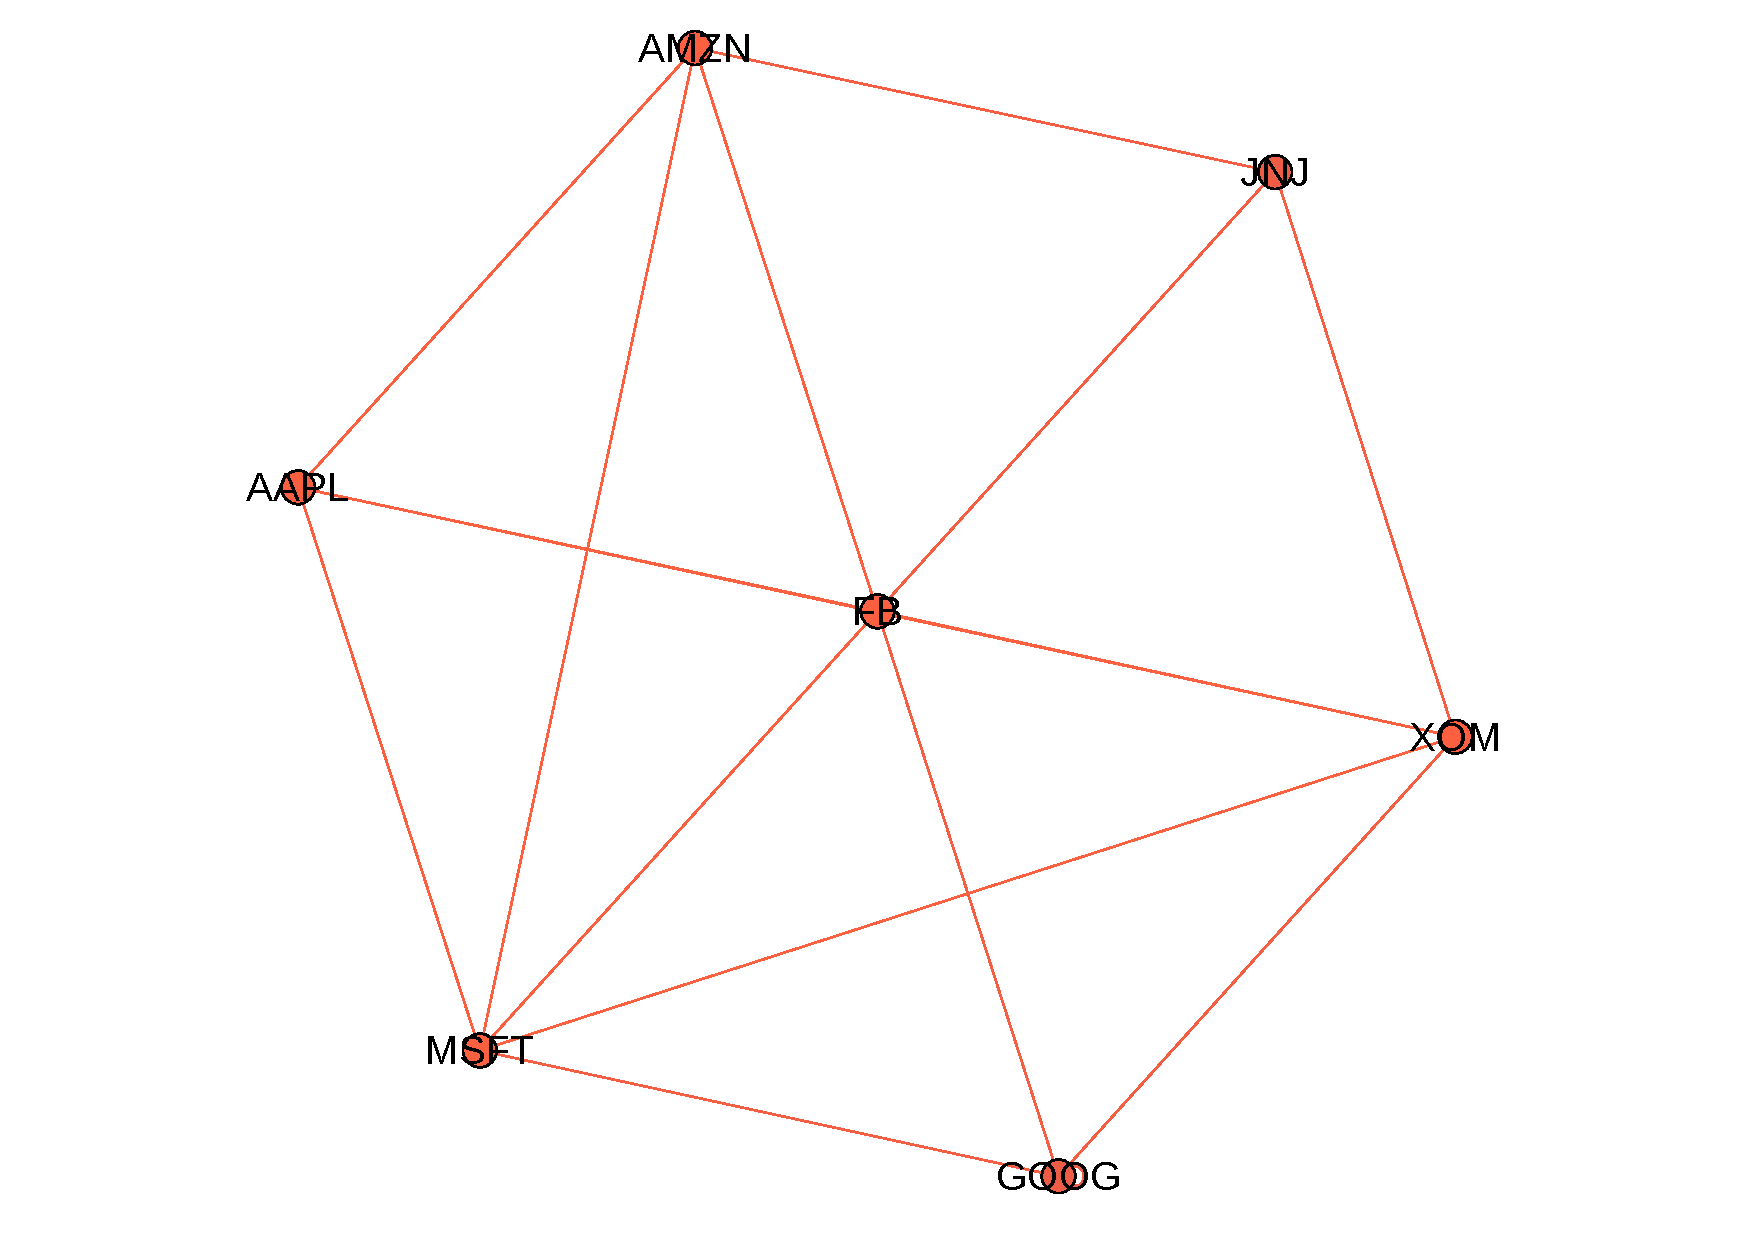
\includegraphics[width=\textwidth]{figures/Intro/ExampleNetwork.pdf}

      \caption{
      This figure contains an example of an undirected graph with 7 nodes and 16 edges. This graph is formed from randomly selecting stock symbol tickers from a set of tickers and forming connections randomly. The purpose of this data is solely to demonstrate the basics of network theory. The nodes are defined as circles and have ticker symbols overlaid on them. Edges are formed between nodes with lines between them. Since this is an undirected graph there is no directional information ergo no distinction as to whether one node is connected to another or vice-versa. The only information represented from an undirected graph is that they are connected. Lastly the amount of connections a node has is referred to as degree. So the node \(FB\) has 6 edges or a degree of 6.
      }
      \label{fig:ExampleNetwork}

  \end{figure*}

\begin{figure*}[!htb]
    \centering
     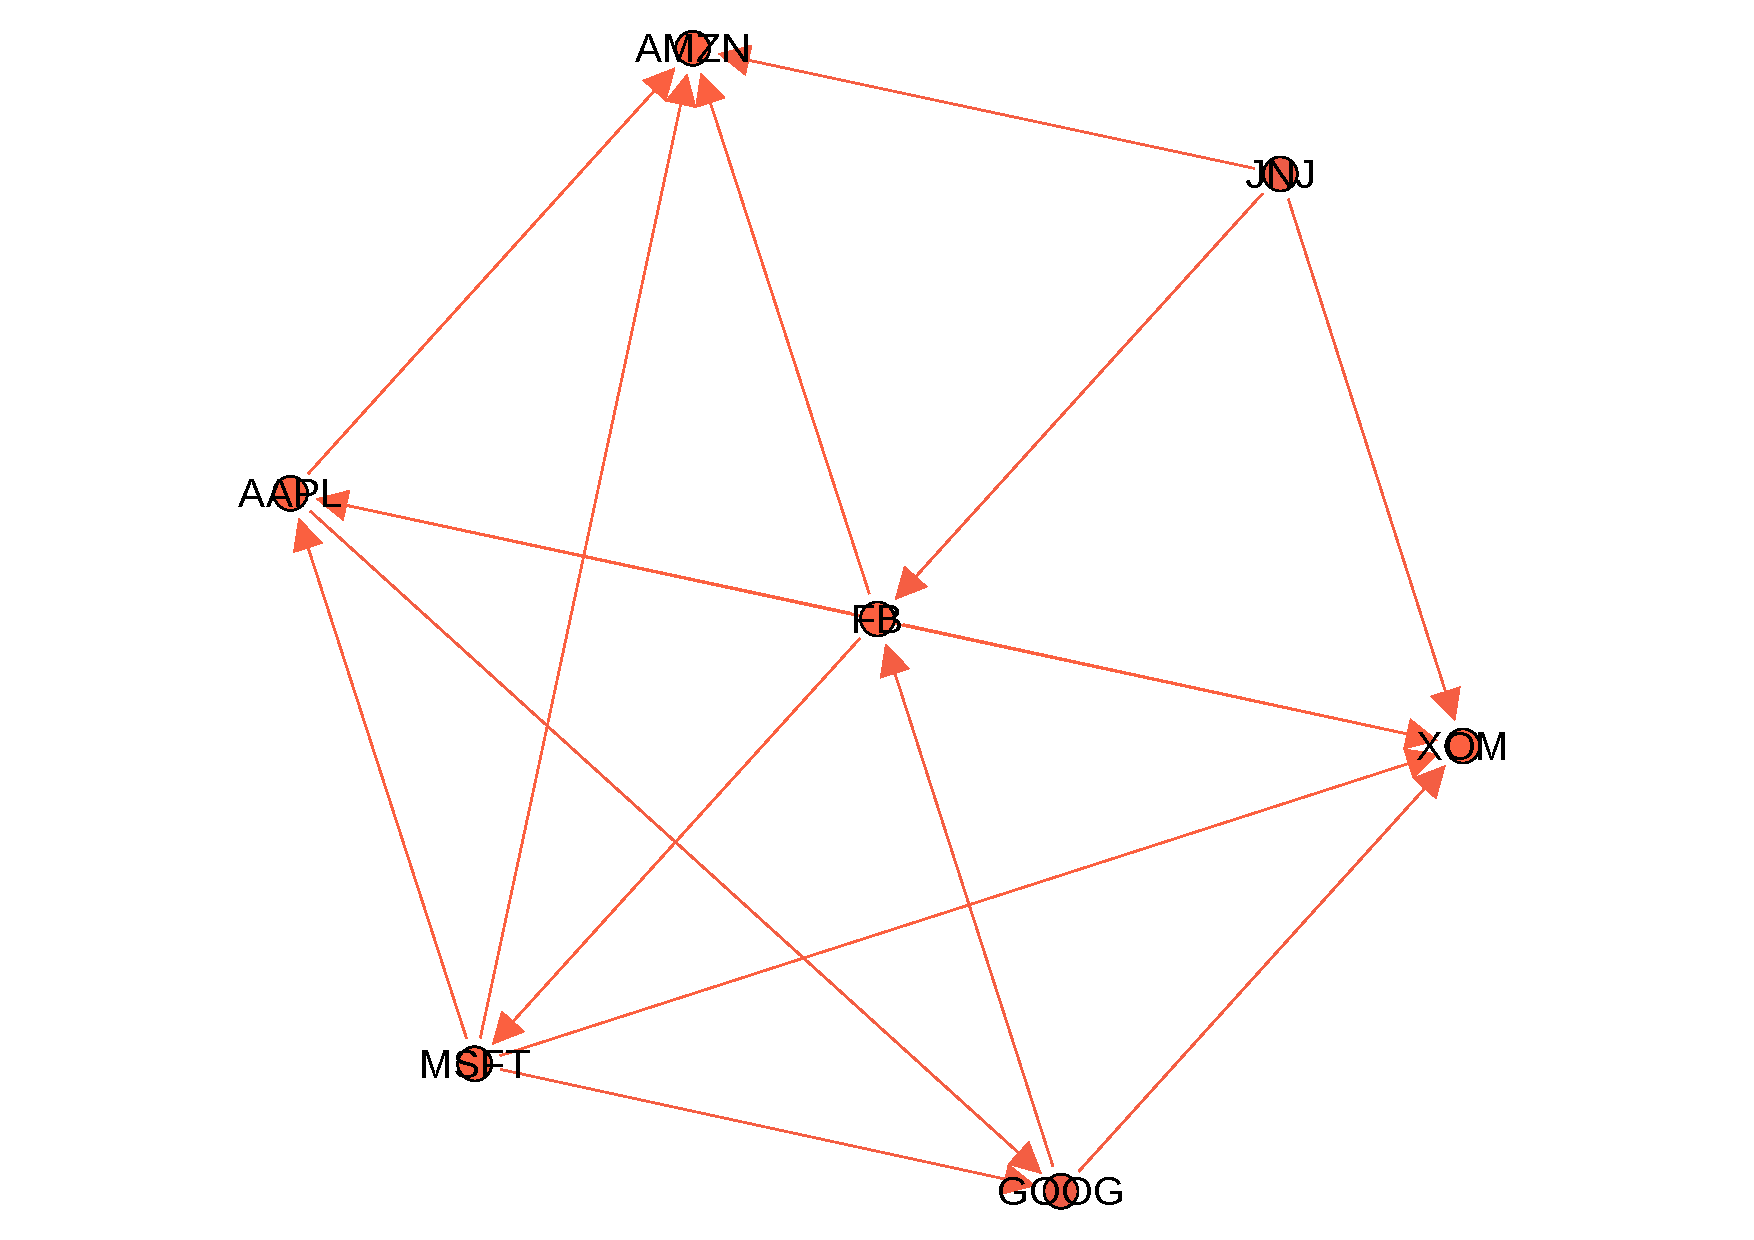
\includegraphics[width=\textwidth]{figures/Intro/ExampleNetworkDirected.pdf}
    \caption{
This graph is nearly identical to the graph in Figure \ref{fig:ExampleNetwork} except this graph is a directed network. This means that it contains directional information between the nodes. This directional information is communicated based on the position of the arrow in a line. For example, the node \(FB\) has an edge to \(MSFT\) however \(MSFT\) does not have an edge to \(FB\). The directional information allows other metrics to be used such as in-degree (which represents the amount of edges directed toward a node) and out-degree (which represents the amount of edges directed away from a node. In this example \(FB\) has an in-degree of 2, an out-degree of 4 and a degree of 6.
      }
	\label{fig:ExampleNetworkDirected}
\end{figure*}



  \begin{figure*}[!htb]
    \centering
      \centering
      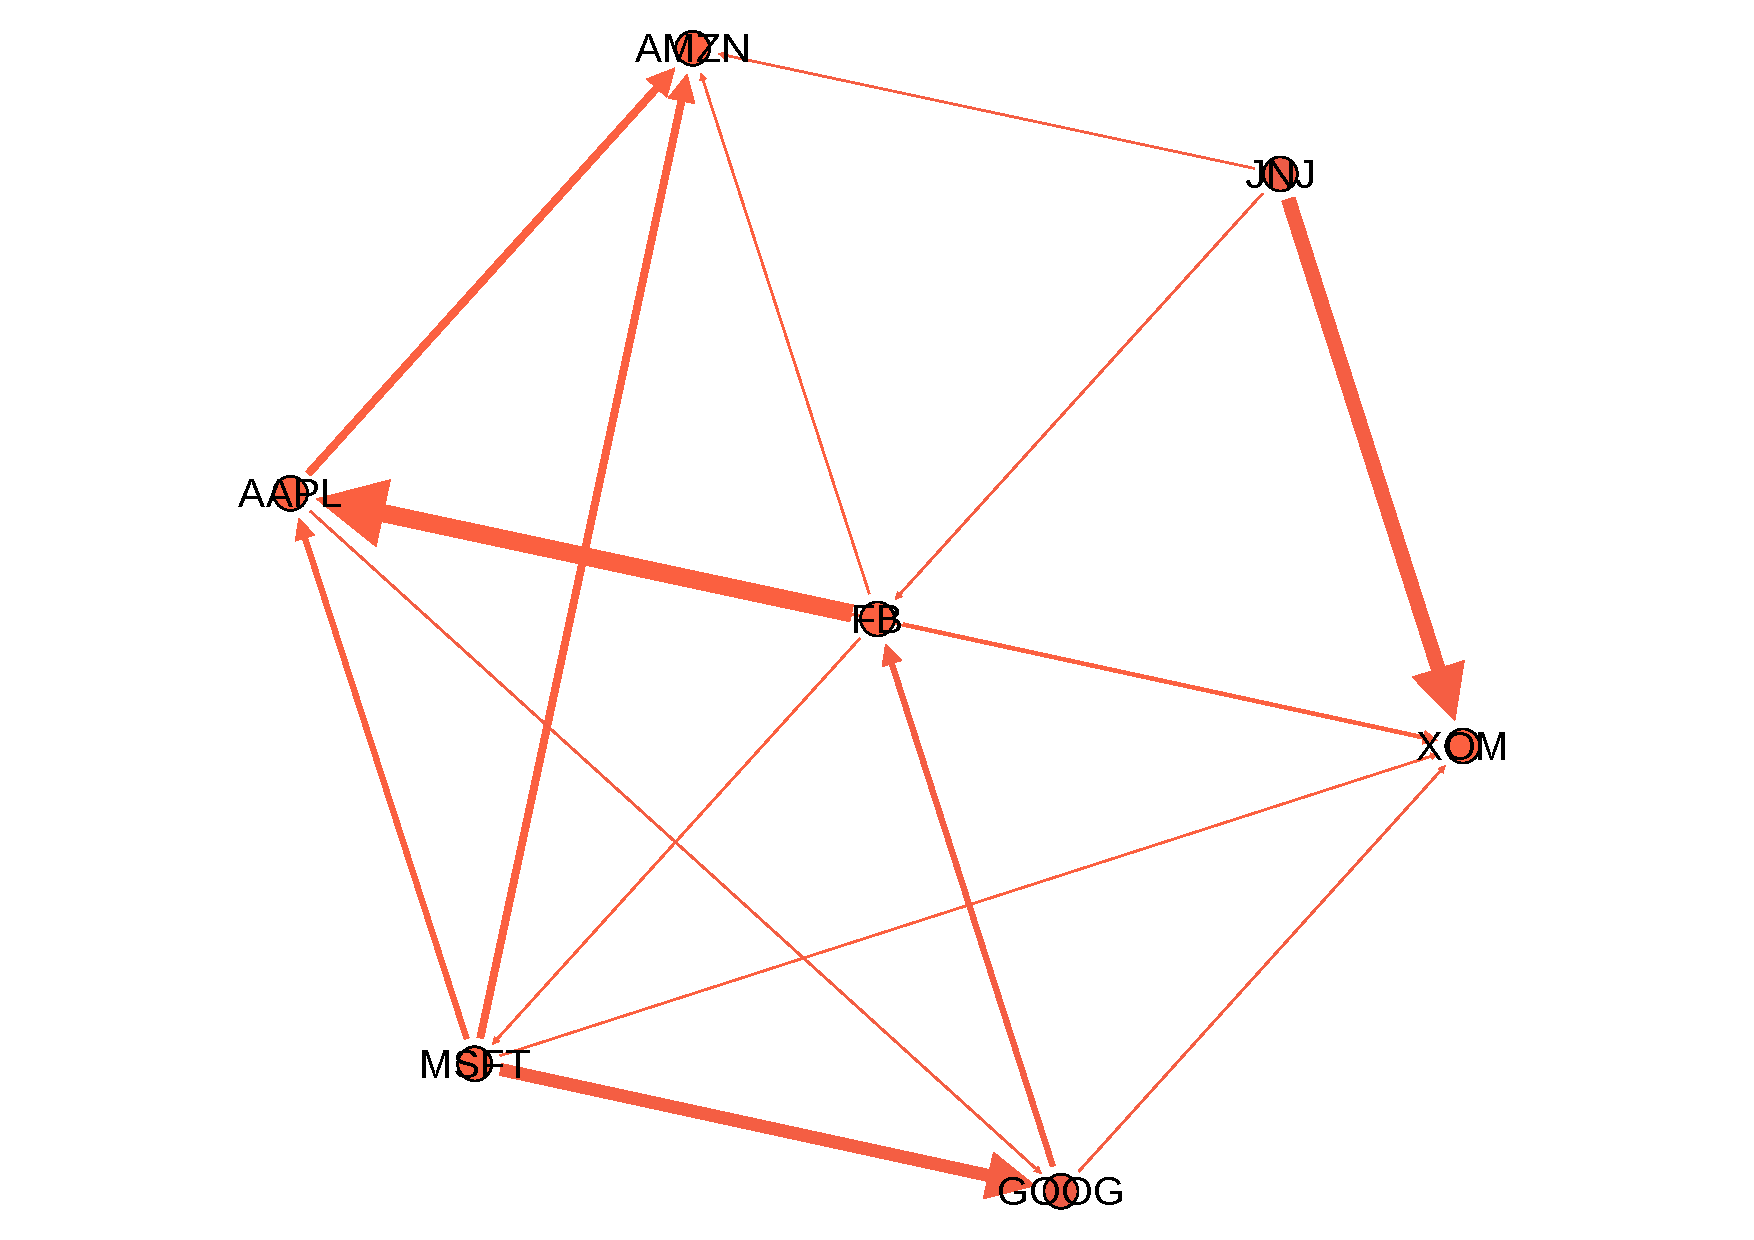
\includegraphics[width=\textwidth]{figures/Intro/ExampleNetworkDirectedWeighted.pdf}
      \caption{A nearly identical graph to the graph in Figure \ref{fig:ExampleNetworkDirected}. This directed graph contains weighted edges where a thick edge represents a high weight value (or strong connection). The smaller the edge weight value the thinner the edge will be.  Here \(FB\) has a strong connection to \(AAPL\) whereas \(FB\) has a weak connection to \(AMZN\).}
      \label{fig:ExampleNetworkDirectedWeighted}
    
  \end{figure*}

\begin{figure*}[!htb]
    \centering
      \centering
      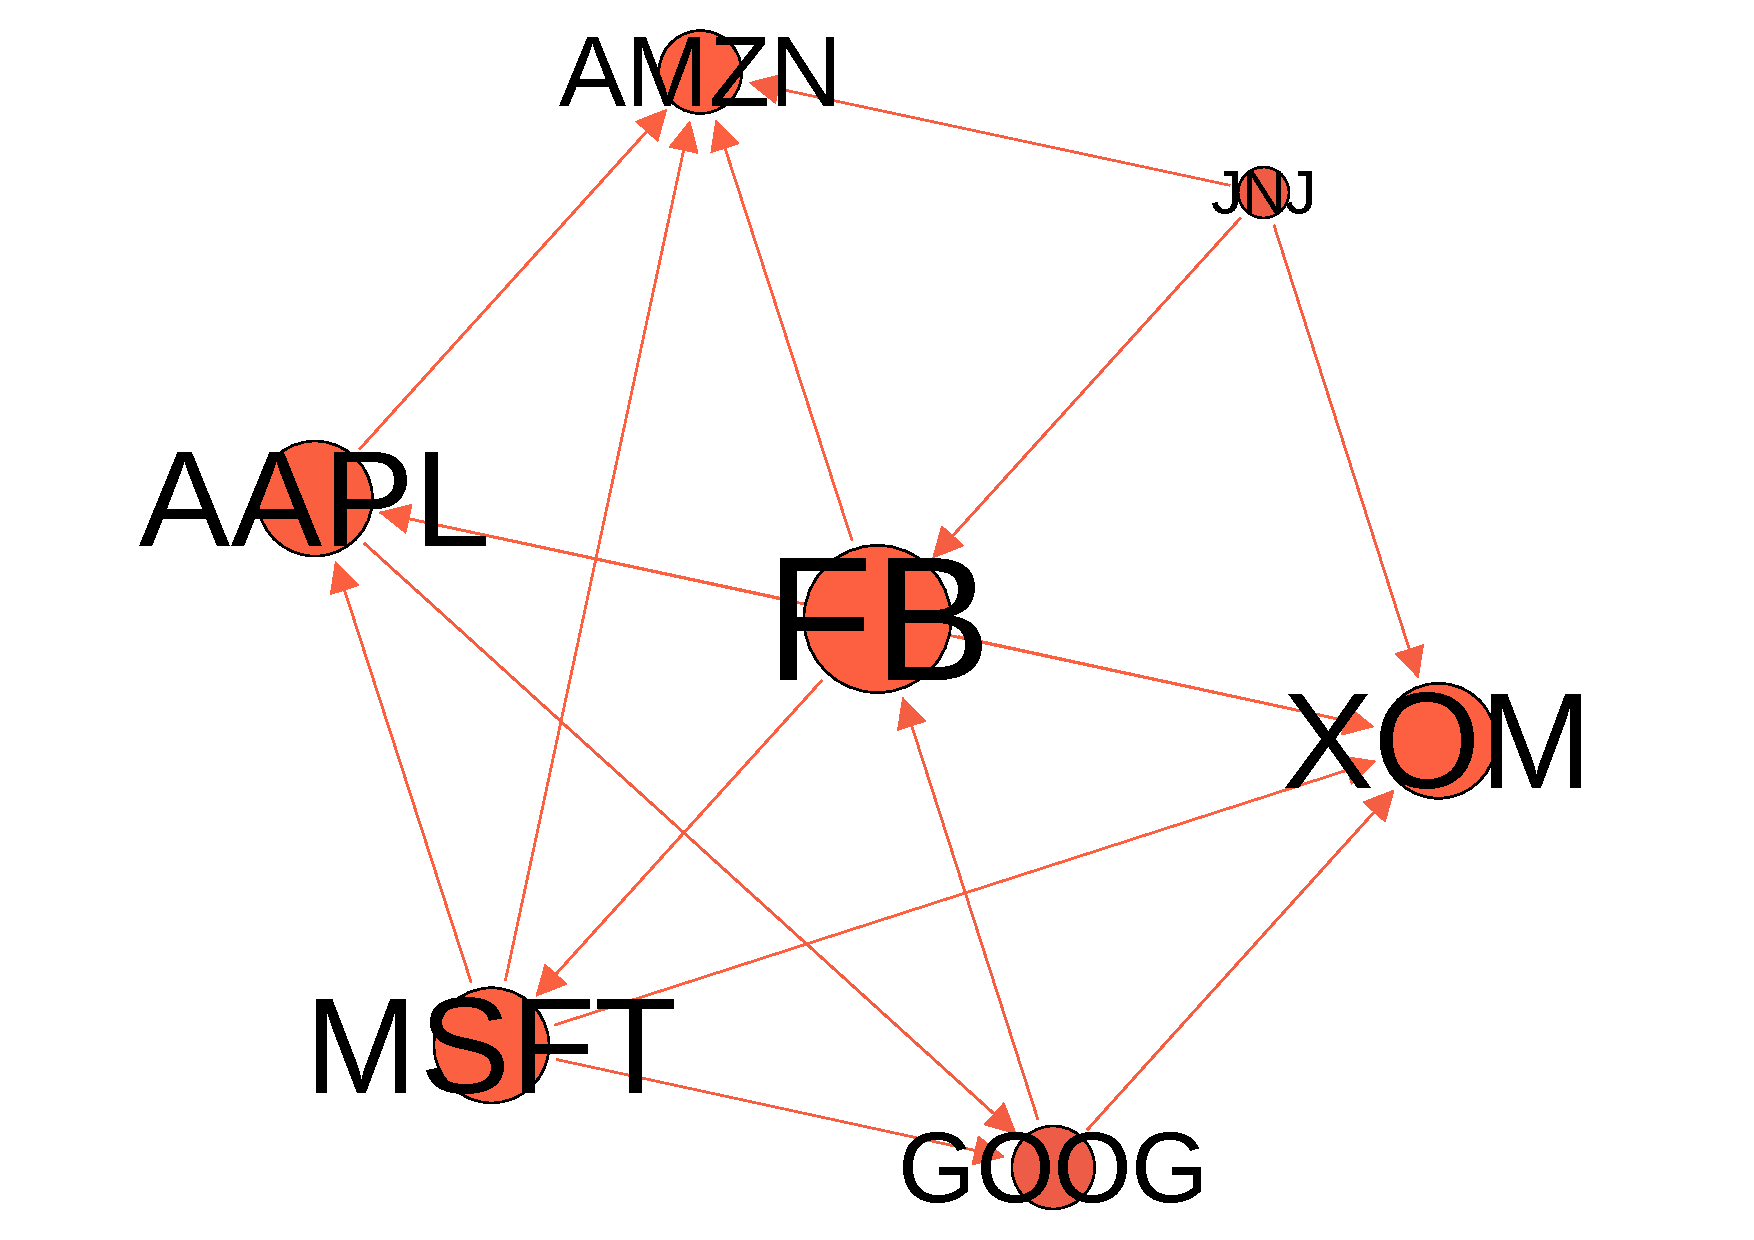
\includegraphics[width=\textwidth]{figures/Intro/ExampleNetworkDegree.pdf}
    \caption{
      A nearly identical graph to the graph in Figure \ref{fig:ExampleNetworkDirected}. Here the node sizes are scaled based on the degree. The higher the degree the larger the node size and consequently the smaller the degree the smaller the node size.
      }
      \label{fig:ExampleNetworkDegree}
  \end{figure*}


\begin{table}[htbp]
\begin{center}
    \begin{tabular}{|p{2cm}|p{1.5cm}|p{1.5cm}|p{1.5cm}|p{1.5cm}|p{1.5cm}|p{1.5cm}|p{1.5cm}|  }
        \hline
         & MSFT & AAPL & AMZN & FB & JNJ &  GOOG & XOM\\
        \hline
        MSFT  & 0 & 1 & 1 & 1  & 0 & 1 & 1 \\
        \hline
        AAPL & 1& 0 & 1 & 1 & 0 & 1 & 1 \\
        \hline
        AMZN & 1 & 1 & 0 & 1 & 1  & 0 & 0 \\
        \hline
        FB & 1 & 1 & 1 & 0  & 1 & 1 & 1 \\
        \hline
        JNJ & 0 & 0 & 1 & 1 & 0 & 0 & 0  \\ 
        \hline
        GOOG & 1 & 1 & 0 & 1 & 0 & 0 & 1 \\
        \hline
        XOM & 1 & 1 & 0 & 1 & 0 & 1 & 0  \\
        \hline
    \end{tabular}
\end{center}
\caption{ 
      This table contains an example of simulated data. This table was formed from randomly selecting stock symbol tickers from a set of tickers. The purpose of this data is solely to demonstrate the basics of network theory. Here the columns and row indicies belong to the selected tickers. The values contain either a 1 to represent if there is a connection between the ticker at a particular row index \(i\)  and the ticker of a particular column \(j\) or a 0 if there is no connection.
}

\label{tab:ExampleTable}
\end{table}

\begin{figure*}[!htb]
    \centering
      \centering
      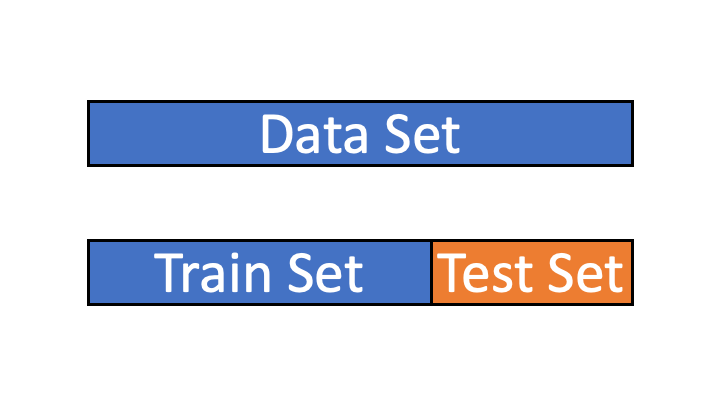
\includegraphics[width=\textwidth]{figures/ppt/TrainTestSplit.png}
    \caption{
      This figure shows how a data set can be partitioned for a supervised machine learning paradigm. The ``Data Set" is partitioned into 2 unequal sets with the``Train Set" having more data assigned to it than the ``Test Set". The ``Train Set" and ``Test Set" ratios can vary and is typically determined by the practitioner. There are many ways to partition the data for the train and test sets. For example the dataset can be partitioned sequentially from the data, or form partitions based on the data being randomly sampled.
      }
\label{fig:TrainTestSplit}

  \end{figure*}


\begin{figure*}[!htb]
    \centering
      \centering
      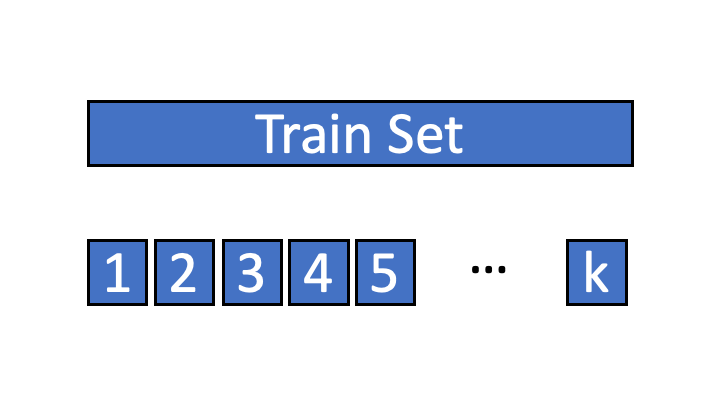
\includegraphics[width=\textwidth]{figures/ppt/KFoldValidation.png}
    \caption{
	``Train Set" here represents ``Train Set" in Figure \ref{fig:TrainTestSplit}. In this figure the data is split into \(k\) folds. How the \(k\) folds are created can vary. A common technique is to randomly divide the ``Train Set" observations into \(k\) equal folds.
      }
     \label{fig:KFoldValidation}
  \end{figure*}

\begin{figure*}[!htb]
    \centering
      \centering
      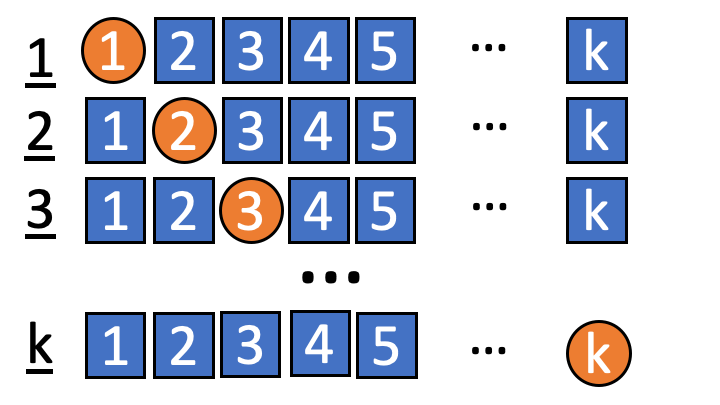
\includegraphics[width=\textwidth]{figures/ppt/KFoldValidationExplain.png}
     
    
    \caption{
	This figure breaks down how \(k\)-Fold Cross Validation works. These folds are created from ``Train Set" in Figure \ref{fig:KFoldValidation}. For the first iteration (where you see 1 underlined), the 1st fold (circle labeled 1) is used to assess the models ability and the remaining folds (squares) are used to train the model. The 2nd iteration follows the same procedure as the 1st except only the 2nd fold is withheld and the other folds are used. This repeats \(k\) times.
      }
\label{fig:KFoldValidationExplain}
  \end{figure*}


\begin{figure*}[!htb]
    \centering
      \centering
      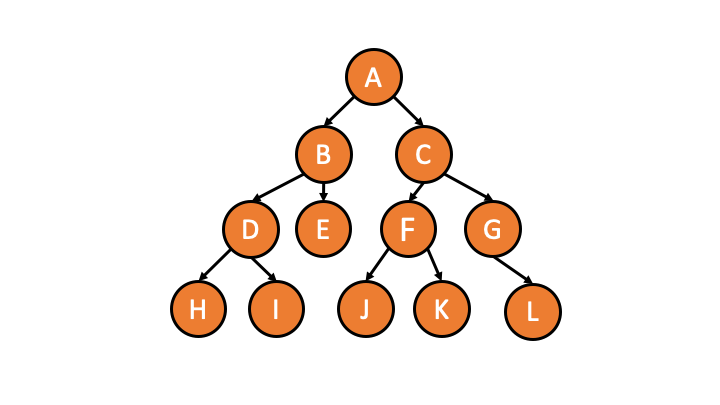
\includegraphics[width=\textwidth]{figures/ppt/DecisionTree.png}

    \caption{
	This figure shows an example of a Decision Tree. This is essentially a graph with no cycles.  Each circle represents a node (the label of the node is a letter inside of the node) and the arrows represent directional edges (branches) to another node. Node \(A\) is the root node of this tree and is where the decision begins. Potential outcomes from the root node lead to different states that are represented in nodes \(B\) and \(C\). \(B\) and \(C\) are the children of \(A\).  Nodes \(B\) and \(C\) have children and their children has children. Nodes \(H, I, E, J, K,\) and \(L\) are the leaf nodes of this tree because they have no children.
      }
      \label{fig:DecisionTree}
  \end{figure*}

\clearpage
\bibliographystyle{plainnat}
\bibliography{thesisbib}